\section{Hardware Setup}
\label{hardware_setup}

% For one-column wide figures use
\begin{figure}[H]
% Use the relevant command to insert your figure file.
% For example, with the graphicx package use
  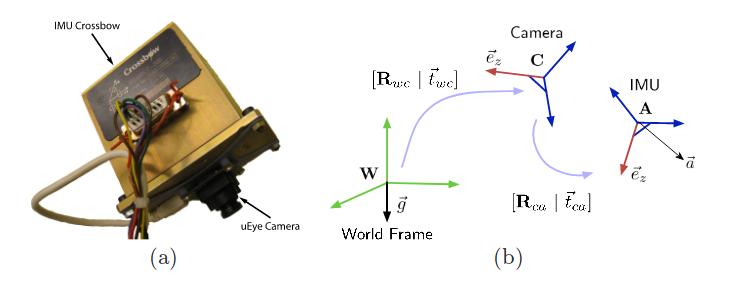
\includegraphics[width=\textwidth]{./figures/imucam.png}
% figure caption is below the figure
\caption{\textbf{a.} Camera/IMU setup. \textbf{b}. Frame transformations between IMU, Camera and World frame.}
\label{fig:setup1}       % Give a unique label
\end{figure}

This section goes through the hardware setup used in the research paper. USB uEye UI-122xLE fisheye camera was used as the vision input. The camera has a resolution of $752 × 480$ and a frame rate up to 87fps. Motion blur was minimized due to the high dynamic range and global shutter of the camera. VG400CC-200 solid state gyro which includes a tri-axial gyroscope and tri-axial accelerometer was used. It has an output frequency of 75 Hz with an input range of $\pm$10g and $<1.25mg$ resolution. The IMU outputs acceleration around its 3-axis along with yaw, pitch and roll.
